\subsection{Neural experiment definitions and audit}
\label{app:empirical-details}
\paragraph{Training objective and sweep aggregation.}
The CNN and MLP use a fixed subset of 8,192 CIFAR-10 training examples.
The objective is the example mean of the sum of squared errors over ten outputs;
the optimizer is SGD without momentum, weight decay, clipping, or added target noise.
The MLP has two hidden layers of width 512 with SiLU activations and 1,841,162 parameters;
the CNN has three convolutional layers with SiLU activations.
Figure~\ref{fig:neural-grids} retains every batch size in
$\{8,32,128,512,2048,4096\}$ and every tested step size for the two architectures:
$\{0.04,0.08,0.16\}$ for the CNN and $\{0.01,0.02,0.04\}$ for the MLP.
Each cell averages three run-level estimates, computed after pooling that run's
last three available checkpoint probe sets. The checkpoint horizons vary across runs and cells.
The reported harmonic statistic is therefore the mean of run-level harmonic statistics,
not the harmonic statistic of a pooled mixture across runs.
All 72 displayed means were recomputed from the immutable saved gains and agree with the
published numerical audit to within $2\times10^{-12}$.
Finite inverse-moment estimates do not establish finiteness of the population inverse moment;
rare gains near zero can dominate that quantity.

\paragraph{Four diagnostic objects.}
For a fixed reference axis $q$, the signed scalar compression is
$a_q=1-\eta q^\top H_Bq/\|q\|^2$.
Its moment estimates use $|a_q|$: $\widehat M_q(p)=\operatorname{mean}|a_q|^p$,
$\widehat\Lambda_q=\operatorname{mean}\log|a_q|$, and
$\widehat H_q=1/\widehat M_q(-1)$.
This differs from the reset-axis norm $\|(I-\eta H_B)q\|/\|q\|$,
which retains the orthogonal part of the update.
Both differ from a continuously propagated tangent vector
$v_{t+1}=(I-\eta H_{B_t}(\theta_t))v_t$.
The plotted cumulative tangent growth sums the log normalization factors while preserving
the transported direction after every update. Three initializations are used: the leading
Ritz vector, the full-data gradient, and a random direction.
Multiple initializations are an empirical check and do not certify an asymptotic top exponent.

\paragraph{Continuation design and fixed frames.}
Four 4,096-update continuations start from retained reference weights:
CNN discovery and confirmation streams at $B=128$, $\eta=0.08$ (reference update 20,000),
and MLP random-reshuffling and iid-subset streams at $B=4096$, $\eta=0.04$
(reference update 10,001). These are fresh continuations, not bit-identical RNG resumes.
Each iid minibatch is a uniform subset without replacement internally; batches are sampled independently across updates.
The 8,192-example training set forms two batches per MLP reshuffling epoch, making the iid control essential.
Four axes are held fixed: a full-data leading Ritz vector, the full-data gradient,
and two random vectors orthogonalized against the Ritz vector.
The MLP leading Ritz estimate uses 30 fully reorthogonalized Lanczos steps;
its eigenpair residual is $2.80\times10^{-7}$ relative to the Rayleigh value $68.1030$.
This certifies a small eigenpair residual, not global extremality.
The reference state and all directions are reused by hash.

\paragraph{Window selection and shape checks.}
Every fixed coordinate is examined at widths 64, 128, 256, 512, and 1,024 updates,
with 50\% overlap. Raw coordinates are primary; detrending is diagnostic only.
The screen requires exactly two prominent KDE maxima at bandwidth factors
$0.7,1,1.4$ times $n^{-1/5}$ times the window standard deviation,
peak prominence at least 15\% of the density maximum, separation at least 0.8 standard deviations,
a valley below 80\% of the smaller peak, and at least 10\% of observations on either side.
This is a descriptive screen, not a calibrated hypothesis test for dependent data.
The displayed MLP interval is the first 512 updates of the late half, updates 2048--2559;
it is an illustrative post-run display choice and also passes the broader bandwidth factor two.
The same top-direction screen passes all 31 windows of width 256, all 15 windows of width 512,
and all seven windows of width 1,024, under both MLP samplers.
These overlapping counts are not independent replications.
Fixed-gradient coordinates are more sensitive to window length; changing centers and amplitudes can
merge lobes when a longer interval is pooled.
Lag-one correlation and ordered traces remain essential: phase slips can weaken a global even/odd split
while the process remains strongly alternating.

\paragraph{Paired-state probes and precision.}
At the initial state, 128 independent minibatches estimate the conditional compression laws.
At each adjacent pair of updates $512k$ and $512k+1$, $k=0,\ldots,7$,
the same 24 fresh minibatches probe both states; these probes do not alter training.
For the iid MLP pair starting at update 2048, the fixed leading-axis harmonic gains are
$1.17495$ and $0.55872$.
Thus the observed lobes cannot be assigned one invariant harmonic regime along this axis.
Training and Hessian products use float32 with TF32 disabled, with float64 reductions for
coordinates, Rayleigh quotients, and norm ratios.
Sparse same-state float64 derivative comparisons have a maximum MLP log-gain discrepancy
of $1.77\times10^{-7}$; this is a local derivative check rather than a global propagation error bound.
An explicit small-network Hessian comparison and same-minibatch finite-difference check also pass.

\begin{figure}[t]
  \centering
  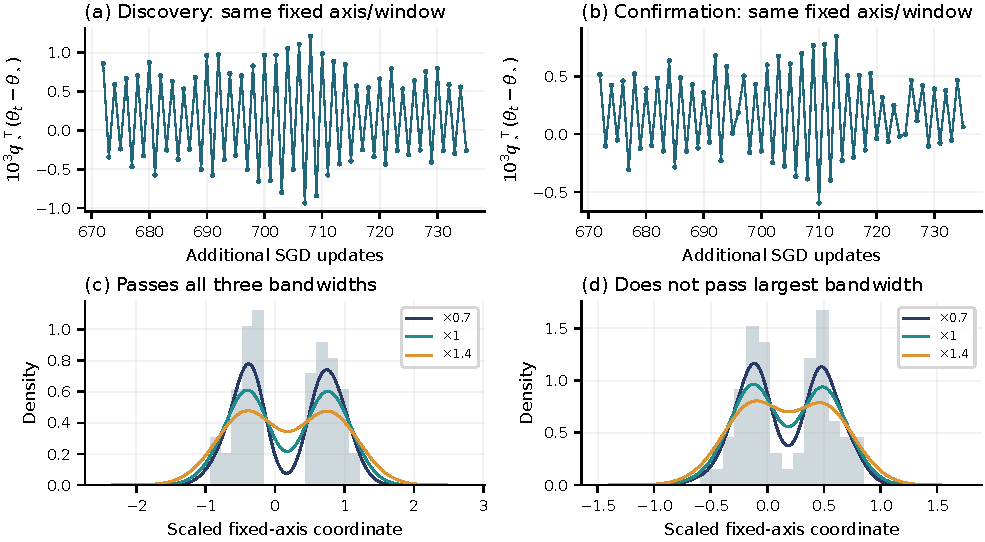
\includegraphics[width=\linewidth]{figures/empirical_cnn_confirmation.pdf}
  \caption{\textbf{A CNN short-window candidate does not confirm.}
  The discovery-only procedure selects the leading fixed axis and updates 672--735;
  the identical relative window is examined in a separate batch stream from the same parent checkpoint.
  Both time traces are shown alongside raw occupancy densities.
  The confirmation density has two prominent peaks at bandwidth factors $0.7$ and $1$,
  but only one at factor $1.4$, failing the fixed screen.
  A visually suggestive short-window histogram alone is therefore insufficient evidence.}
  \label{fig:cnn-confirmation}
\end{figure}
